\documentclass[11pt,a4paper]{article}
\usepackage[margin=21mm,headheight=16pt]{geometry}
\usepackage{fontspec}\setmainfont{Noto Serif}\setsansfont{Noto Sans}\setmonofont{Noto Sans Mono}
\usepackage{polyglossia}\setdefaultlanguage{turkish}
\usepackage{amsmath,amssymb,mathtools,graphicx,xcolor,booktabs,tabularx,array,enumitem}
\usepackage[most]{tcolorbox}\usepackage{fancyhdr,titlesec,needspace}
\usepackage[unicode,hidelinks,breaklinks]{hyperref}\usepackage{bookmark}
\definecolor{ink}{HTML}{18233A}\definecolor{accent}{HTML}{545AC4}\definecolor{green}{HTML}{087E66}\definecolor{paper}{HTML}{F3F5FA}
\color{ink}\setlength{\parindent}{0pt}\setlength{\parskip}{7pt}\linespread{1.10}
\setlength{\emergencystretch}{3em}\allowdisplaybreaks
\setlist{topsep=4pt,itemsep=4pt,leftmargin=*}
\pagestyle{fancy}\fancyhf{}\fancyhead[L]{\sffamily\small MÜHENDİSLİK MATEMATİĞİ}\fancyhead[R]{\sffamily\small Ders çalışma notları}\fancyfoot[L]{\sffamily\scriptsize Fotoğraflar + müfredat | 8 Kasım 2026}\fancyfoot[R]{\sffamily\thepage}
\titleformat{\section}{\Large\sffamily\bfseries\color{accent}}{\thesection}{.6em}{}
\titleformat{\subsection}{\large\sffamily\bfseries}{\thesubsection}{.6em}{}
\tcbset{enhanced,breakable,boxrule=.4pt,arc=2mm,left=3mm,right=3mm,top=2mm,bottom=2mm,before skip=8pt,after skip=8pt,fonttitle=\sffamily\bfseries,colback=paper,colframe=accent,coltitle=white}
\newcommand{\notebox}[2]{\begin{tcolorbox}[title={#1},colframe=accent!70!black]#2\end{tcolorbox}}
\hypersetup{pdfauthor={Mühendislik Matematiği Çalışma Atölyesi},pdfsubject={Ders fotoğrafları ve altı başlıklı müfredata göre özgün Türkçe çalışma notları}}
\begin{document}

\hypersetup{pdftitle={Vektör fonksiyonları, eğriler ve hareket}}
{\sffamily\small\color{accent} ÇALIŞMA ATÖLYESİ / KONU 03\par}
\vspace{8mm}
{\Huge\sffamily\bfseries\raggedright\hyphenpenalty=10000 Vektör fonksiyonları, eğriler ve hareket\par}
\vspace{3mm}
{\large Vektörel limit, türev ve integral; yay uzunluğu, Frenet çatısı, eğrilik, hız ve ivme.\par}
\vspace{4mm}\hrule\vspace{4mm}\subsection*{Bu bölümün hedefleri}\begin{itemize}
\item Vektör fonksiyonunu bileşenlerinden incelemek; eğriyi ve yönünü belirlemek.
\item Teğet, normal, binormal ve eğriliği hesaplamak.
\item Hız vektörünü süratten ayırmak; ivmeyi teğetsel ve normal bileşenlerine ayırmak.\end{itemize}
{\small\tableofcontents}\clearpage
\section{Vektör değerli fonksiyon ve tanım kümesi}
Bir gerçek parametreyi bir vektöre gönderen fonksiyon \(\mathbf r:I\to\mathbb R^3\) biçimindedir. \(\mathbf r(t)=(x(t),y(t),z(t))\) konum vektörünün ucu bir uzay eğrisi çizer. Parametre zaman olabilir; ancak her parametrizasyon fiziksel zaman değildir. Tanım kümesi, üç bileşenin tanım kümelerinin kesişimidir.

\Needspace{10\baselineskip}\begin{tcolorbox}[title={Örnek 3.1 | Defterdeki tanım kümesi örneği},colframe=accent]\(\mathbf F(t)=(t+1,\ln(1-t),\sqrt{4-t^2})\) için tanım kümesini bulunuz.
\par\vspace{1mm}{\scriptsize\sffamily Ders fotoğrafından | \nolinkurl{IMG-20261009-WA0016.jpg}}\end{tcolorbox}
\begin{tcolorbox}[title={Adım adım çözüm},colback=green!3!white,colframe=green]\begin{enumerate}
\item İlk bileşen tüm gerçek sayılarda tanımlıdır. Logaritma için \(1-t>0\), yani \(t<1\). Karekök için \(-2\le t\le2\).
\item Koşulları birlikte sağlamak gerekir: \(I=[-2,1)\). \(-2\) kabul edilir, çünkü kök sıfır olabilir; 1 kabul edilmez, çünkü logaritma argümanı sıfır olamaz.
\end{enumerate}\end{tcolorbox}
Vektör fonksiyonlarında toplama, skalerle çarpma, skaler ve vektörel çarpım her t anında uygulanır. Skaler çarpımın çıktısı gerçek sayılı bir fonksiyon; vektörel çarpımın çıktısı yeniden vektör fonksiyonudur.

\Needspace{10\baselineskip}\begin{tcolorbox}[title={Örnek 3.2 | Vektör fonksiyonlarıyla işlemler},colframe=accent]\(\mathbf F=(t,t^2,t^3)\), \(\mathbf G=(1-t,1+t^2,t)\). Toplamı, skaler ve vektörel çarpımı bulunuz.
\par\vspace{1mm}{\scriptsize\sffamily Ders fotoğrafından | \nolinkurl{IMG-20261009-WA0017.jpg}}\end{tcolorbox}
\begin{tcolorbox}[title={Adım adım çözüm},colback=green!3!white,colframe=green]\begin{enumerate}
\item \(\mathbf F+\mathbf G=(1,1+2t^2,t^3+t)\).
\item \(\mathbf F\cdot\mathbf G=t(1-t)+t^2(1+t^2)+t^4=t+2t^4\).
\item \(\mathbf F\times\mathbf G=(-t^5,t^3-t^4-t^2,t+2t^3-t^2)\). Her bileşen determinant açılımından gelir.
\end{enumerate}\end{tcolorbox}
\section{Limit ve süreklilik bileşenlere ayrılır}

{\small\[
\lim_{t\to t_0}\mathbf r(t)=(L_1,L_2,L_3)\quad\Longleftrightarrow\quad\lim x(t)=L_1,\ \lim y(t)=L_2,\ \lim z(t)=L_3.
\]}
Bu eşdeğerlik sonlu boyutta normla yakınsamanın koordinat yakınsamasıyla aynı olmasından gelir. Süreklilik için fonksiyonun noktada tanımlı olması, limitin var olması ve limitin o noktadaki değere eşit olması gerekir. Tek bileşendeki bir sıçrama bütün vektör fonksiyonunu süreksiz yapar.

\Needspace{10\baselineskip}\begin{tcolorbox}[title={Örnek 3.3 | Defterdeki limit işlemleri},colframe=accent]\(\mathbf F(t)=(\sin t,\cos t,1+t)\), \(\mathbf G(t)=(\cos2t,\sin3t,e^t+1)\) için t sıfıra giderken skaler ve vektörel çarpım limitlerini bulunuz.
\par\vspace{1mm}{\scriptsize\sffamily Ders fotoğrafından | \nolinkurl{IMG-20261009-WA0019.jpg}}\end{tcolorbox}
\begin{tcolorbox}[title={Adım adım çözüm},colback=green!3!white,colframe=green]\begin{enumerate}
\item \(\mathbf F\to(0,1,1)\), \(\mathbf G\to(1,0,2)\).
\item Skaler çarpım limiti \((0,1,1)\cdot(1,0,2)=2\). Vektörel çarpım limiti \((0,1,1)\times(1,0,2)=(2,1,-1)\).
\end{enumerate}\end{tcolorbox}
\Needspace{10\baselineskip}\begin{tcolorbox}[title={Örnek 3.4 | Tam kısım içeren süreklilik},colframe=accent]\(\mathbf F(t)=(|t|+1,t\lfloor t\rfloor,2+t^2)\) fonksiyonu 0 ve 1 noktalarında sürekli midir?
\par\vspace{1mm}{\scriptsize\sffamily Ders fotoğrafından | \nolinkurl{IMG-20261009-WA0019.jpg}}\end{tcolorbox}
\begin{tcolorbox}[title={Adım adım çözüm},colback=green!3!white,colframe=green]\begin{enumerate}
\item İlk ve üçüncü bileşen her yerde süreklidir. İkinci bileşen 0 yakınında solda \(-t\), sağda 0 olur; iki yandan limit 0, değer de 0. Dolayısıyla 0 noktasında süreklidir.
\item 1 yakınında solda ikinci bileşen 0, sağda t olur. Limitler 0 ve 1 olduğundan 1 noktasında süreksizdir.
\end{enumerate}\end{tcolorbox}
\section{Eğriyi, izini ve yönünü ayırt etmek}
Parametrik denklemlerden t yok edilerek eğrinin hangi yüzeylerin üzerinde bulunduğu anlaşılır. Ancak parametreyi yok etmek yönü ve kaç kez dolaşıldığını kaybettirir. Aynı geometrik iz farklı parametrizasyonlarla farklı hızlarda ve ters yönlerde taranabilir.

\Needspace{10\baselineskip}\begin{tcolorbox}[title={Örnek 3.5 | Çember ve helis},colframe=accent]\(\mathbf r(t)=(a\cos t,a\sin t,0)\) ile \(\mathbf h(t)=(\cos t,\sin t,3t)\) eğrilerini yorumlayınız.
\par\vspace{1mm}{\scriptsize\sffamily Ders fotoğrafından | \nolinkurl{IMG-20261009-WA0022.jpg}}\end{tcolorbox}
\begin{tcolorbox}[title={Adım adım çözüm},colback=green!3!white,colframe=green]\begin{enumerate}
\item İlkinde \(x^2+y^2=a^2\), \(z=0\). \(a>0\) ve \(0\le t\le2\pi\) için pozitif z yönünden bakıldığında çember saat yönünün tersine bir tur taranır.
\item İkincide \(x^2+y^2=1\); yükseklik t ile artar. Bir turda t, \(2\pi\) artar ve yükseklik \(6\pi\) değişir. Bu eğri bir helistir.
\end{enumerate}\end{tcolorbox}
Bir parametrizasyon sürekli, parçalı türevlenebilir olabilir. Düzgünlük için ilgili aralıkta türevin sürekli ve \(\mathbf r\,\prime(t)\ne\mathbf0\) olması istenir. Türevin sıfır olduğu bir parametrizasyon noktasında standart birim teğet formülü doğrudan uygulanmaz; eğrinin geometrisi ayrıca incelenir.

\Needspace{10\baselineskip}\begin{tcolorbox}[title={Örnek 3.6 | Parçalı düzgün eğri},colframe=accent]\(\mathbf r(t)=(a\cos t,a|\sin t|,0)\), \(-2\pi\le t\le2\pi\), \(a>0\) için düzgünlük nasıldır?
\par\vspace{1mm}{\scriptsize\sffamily Ders fotoğrafından | \nolinkurl{IMG-20261015-WA0038.jpg}}\end{tcolorbox}
\begin{tcolorbox}[title={Adım adım çözüm},colback=green!3!white,colframe=green]\begin{enumerate}
\item \(\sin t\) işaret değiştirdiğinde mutlak değerin türevi değişir. \(t=k\pi\) noktalarında tek taraflı teğet vektörler uyuşmaz; verilen parametrizasyon düzgün değildir.
\item Aradaki açık aralıklarda türev vardır ve normu a olur. Dolayısıyla sonlu sayıda parçaya ayrılarak parçalı düzgün kabul edilir. İz üst yarım çemberdir; birden fazla kez taranır.
\end{enumerate}\end{tcolorbox}
\section{Türev, teğet doğrusu ve çarpım kuralları}
\(\Delta\mathbf r/\Delta t\), iki konum arasındaki kirişin zamana oranıdır. Limitte anlık değişim vektörüne dönüşür. \(\mathbf r\,\prime(t_0)\ne\mathbf0\) ise bu vektör eğrinin o noktadaki teğet yönüdür. Teğet doğrusu yeni bir parametreyle \(\mathbf q(s)=\mathbf r(t_0)+s\mathbf r\,\prime(t_0)\) olarak yazılır.


{\small\[
\mathbf r\,\prime(t)=\lim_{h\to0}\frac{\mathbf r(t+h)-\mathbf r(t)}h=(x\prime(t),y\prime(t),z\prime(t)).
\]}

{\small\[
\begin{aligned}(\phi\mathbf F)\prime&=\phi\prime\mathbf F+\phi\mathbf F\prime,\\(\mathbf F\cdot\mathbf G)\prime&=\mathbf F\prime\cdot\mathbf G+\mathbf F\cdot\mathbf G\prime,\\(\mathbf F\times\mathbf G)\prime&=\mathbf F\prime\times\mathbf G+\mathbf F\times\mathbf G\prime.\end{aligned}
\]}
\Needspace{10\baselineskip}\begin{tcolorbox}[title={Örnek 3.7 | Dersteki temel türevler},colframe=accent]\(\mathbf F(t)=(t,t^2,t^3)\) ve \(\mathbf G(t)=(t\ln t-t,e^t,e^{-t})\) türevlerini bulunuz.
\par\vspace{1mm}{\scriptsize\sffamily Ders fotoğrafından | \nolinkurl{IMG-20261023-WA0058.jpg}}\end{tcolorbox}
\begin{tcolorbox}[title={Adım adım çözüm},colback=green!3!white,colframe=green]\begin{enumerate}
\item Bileşenler ayrı türevlenir: \(\mathbf F\prime=(1,2t,3t^2)\).
\item İkinci fonksiyonun ilk bileşeninde çarpım kuralı \((t\ln t-t)\prime=\ln t+1-1=\ln t\) verir. \(\mathbf G\prime=(\ln t,e^t,-e^{-t})\), \(t>0\).
\end{enumerate}\end{tcolorbox}
\Needspace{10\baselineskip}\begin{tcolorbox}[title={Örnek 3.8 | Zincir kuralı içeren vektör türevi},colframe=accent]\(\mathbf F(t)=(\arcsin(4t),-3\arctan(2t-1),7\ln(3t^2))\) türevini bulunuz.
\par\vspace{1mm}{\scriptsize\sffamily Ders fotoğrafından | \nolinkurl{IMG-20261023-WA0058.jpg}}\end{tcolorbox}
\begin{tcolorbox}[title={Adım adım çözüm},colback=green!3!white,colframe=green]\begin{enumerate}
\item İlk bileşenin türevi \(4/\sqrt{1-16t^2}\); ikincinin türevi \(-6/[1+(2t-1)^2]\).
\item Üçüncü bileşen \(7(6t)/(3t^2)=14/t\). Türev formüllerinin ortak geçerlilik aralığı \(-1/4<t<1/4\), \(t\ne0\). Fonksiyon uçlarda tanımlı olsa da bu türevler uçlarda sonlu değildir.
\end{enumerate}\end{tcolorbox}
\Needspace{10\baselineskip}\begin{tcolorbox}[title={Örnek 3.9 | Tahtadaki özdeşliğin kanıtı},colframe=accent]\([\mathbf F(t)\times\mathbf F\prime(t)]\prime=\mathbf F(t)\times\mathbf F\prime\prime(t)\) olduğunu gösteriniz.
\par\vspace{1mm}{\scriptsize\sffamily Ders fotoğrafından | \nolinkurl{IMG-20261023-WA0058.jpg}}\end{tcolorbox}
\begin{tcolorbox}[title={Adım adım çözüm},colback=green!3!white,colframe=green]\begin{enumerate}
\item Çarpım kuralı sol tarafı \(\mathbf F\prime\times\mathbf F\prime+\mathbf F\times\mathbf F\prime\prime\) yapar.
\item Bir vektörün kendisiyle vektörel çarpımı sıfırdır. İlk terim silinince istenen özdeşlik kalır.
\end{enumerate}\end{tcolorbox}
\section{Vektör fonksiyonlarının integrali}
İntegral de bileşen bileşen hesaplanır. Belirsiz integralde sabit bir vektör \(\mathbf C=(C_1,C_2,C_3)\) eklenir. Tek bir skaler sabiti bütün bileşenlere zorunlu olarak aynı eklemek genel çözümü daraltır. Başlangıç koşulu varsa üç sabit ayrı ayrı belirlenir.


{\small\[
\int_a^b\mathbf r(t)\,dt=\left(\int_a^b x(t)\,dt,\int_a^b y(t)\,dt,\int_a^b z(t)\,dt\right).
\]}
\Needspace{10\baselineskip}\begin{tcolorbox}[title={Örnek 3.10 | Başlangıç koşullu integral},colframe=accent]\(\mathbf r\prime(t)=(2t,e^{3t},4\sin2t)\), \(\mathbf r(0)=(2,1,-2)\). Konumu bulunuz.
\par\vspace{1mm}{\scriptsize\sffamily Ders fotoğrafından | \nolinkurl{IMG-20261015-WA0037.jpg}}\end{tcolorbox}
\begin{tcolorbox}[title={Adım adım çözüm},colback=green!3!white,colframe=green]\begin{enumerate}
\item İntegral \(\mathbf r(t)=(t^2+C_1,e^{3t}/3+C_2,-2\cos2t+C_3)\).
\item Başlangıçtan \(C_1=2,C_2=2/3,C_3=0\). Dolayısıyla \(\mathbf r(t)=(t^2+2,(e^{3t}+2)/3,-2\cos2t)\).
\end{enumerate}\end{tcolorbox}
\Needspace{10\baselineskip}\begin{tcolorbox}[title={Örnek 3.11 | Dersteki belirli integral üçlüsü},colframe=accent]\(\int_0^1(4t^3,3,2(t+1))dt\), \(\int_1^2(6-6t,3\sqrt t,4/t^2)dt\) ve \(\int_{-\pi/4}^{\pi/4}(\sin t,1+\cos t,\sec^2t)dt\) hesaplayınız.
\par\vspace{1mm}{\scriptsize\sffamily Ders fotoğrafından | \nolinkurl{IMG-20261023-WA0058.jpg}}\end{tcolorbox}
\begin{tcolorbox}[title={Adım adım çözüm},colback=green!3!white,colframe=green]\begin{enumerate}
\item İlkinde ilkel fonksiyon \((t^4,3t,t^2+2t)\). Sonuç \((1,3,3)\).
\item İkincide ilkel fonksiyon \((6t-3t^2,2t^{3/2},-4/t)\). Sonuç \((-3,4\sqrt2-2,2)\).
\item Üçüncüde sinüs tek fonksiyon olduğundan ilk bileşen 0. İkinci \(\pi/2+\sqrt2\), üçüncü \(\tan(\pi/4)-\tan(-\pi/4)=2\).
\end{enumerate}\end{tcolorbox}
\section{Yay uzunluğu ve yay parametresi}
Küçük bir zaman aralığında alınan yol yaklaşık \(\|\mathbf r\prime(t)\|dt\) olur. Bu parçaları toplamak integrali verir. Normun integralini almak gerekir; integralin normu genellikle yer değiştirmedir ve yol uzunluğundan küçük olabilir. Eğri tekrar taranırsa integral tekrar gidilen yolu da sayar.


{\small\[
L=\int_a^b\|\mathbf r\prime(t)\|dt,\qquad s(t)=\int_a^t\|\mathbf r\prime(u)\|du,\qquad\frac{ds}{dt}=\|\mathbf r\prime(t)\|.
\]}
\Needspace{10\baselineskip}\begin{tcolorbox}[title={Örnek 3.12 | Dersteki 5-12-13 helisi},colframe=accent]\(\mathbf r(t)=(5\cos t,5\sin t,12t)\), \(0\le t\le2\pi\), uzunluğunu bulunuz.
\par\vspace{1mm}{\scriptsize\sffamily Ders fotoğrafından | \nolinkurl{IMG-20261015-WA0039.jpg}}\end{tcolorbox}
\begin{tcolorbox}[title={Adım adım çözüm},colback=green!3!white,colframe=green]\begin{enumerate}
\item \(\mathbf r\prime=(-5\sin t,5\cos t,12)\); norm \(\sqrt{25\sin^2t+25\cos^2t+144}=13\).
\item \(L=\int_0^{2\pi}13dt=26\pi\). Bu aralıkta \(s=13t\) olduğundan yay parametreli biçim \((5\cos(s/13),5\sin(s/13),12s/13)\), \(0\le s\le26\pi\).
\end{enumerate}\end{tcolorbox}
\section{Frenet çatısı: teğet, normal, binormal}
Birim teğet \(\mathbf T\) hareket yönünü gösterir. \(\mathbf T\) yön değiştiriyorsa türevi teğete diktir; birimleştirilince asal normal \(\mathbf N\) elde edilir. \(\mathbf B=\mathbf T\times\mathbf N\) eğrinin anlık dönme düzlemine diktir. Bu üçlü sağ elli ortonormal bir çatıdır.


{\small\[
\mathbf T=\frac{\mathbf r\prime}{\|\mathbf r\prime\|},\qquad\mathbf N=\frac{\mathbf T\prime}{\|\mathbf T\prime\|},\qquad\mathbf B=\mathbf T\times\mathbf N=\frac{\mathbf r\prime\times\mathbf r\prime\prime}{\|\mathbf r\prime\times\mathbf r\prime\prime\|}.
\]}
\notebox{Geçerlilik koşulu}{\(\mathbf T\) için hız sıfır olmamalıdır. \(\mathbf N\) ve \(\mathbf B\) için ayrıca eğrilik sıfır olmamalıdır. Düz bir doğruda normal ve binormal bu formüllerle tek olarak belirlenmez.}
\Needspace{10\baselineskip}\begin{tcolorbox}[title={Örnek 3.13 | Çemberin Frenet çatısı},colframe=accent]\(\mathbf r(t)=(\cos t,\sin t,0)\) için \(\mathbf T,\mathbf N,\mathbf B\) nedir?
\par\vspace{1mm}{\scriptsize\sffamily Ders fotoğrafından | \nolinkurl{IMG-20261015-WA0034.jpg}}\end{tcolorbox}
\begin{tcolorbox}[title={Adım adım çözüm},colback=green!3!white,colframe=green]\begin{enumerate}
\item \(\mathbf r\prime=(-\sin t,\cos t,0)\) normu 1 olduğundan \(\mathbf T=(-\sin t,\cos t,0)\).
\item \(\mathbf T\prime=(-\cos t,-\sin t,0)\) normu da 1: \(\mathbf N=(-\cos t,-\sin t,0)\).
\item Çarpım \(\mathbf B=(0,0,1)\). Normal merkeze yönelir; binormal sabittir.
\end{enumerate}\end{tcolorbox}
\Needspace{10\baselineskip}\begin{tcolorbox}[title={Örnek 3.14 | Dersteki uzay eğrisinin Frenet üçlüsü},colframe=accent]\(\mathbf r(t)=(e^t,e^{-t},\sqrt2\,t)\) için \(t=0\) anındaki çatıyı bulunuz.
\par\vspace{1mm}{\scriptsize\sffamily Ders fotoğrafından | \nolinkurl{IMG-20261015-WA0040.jpg}}\end{tcolorbox}
\begin{tcolorbox}[title={Adım adım çözüm},colback=green!3!white,colframe=green]\begin{enumerate}
\item \(\mathbf v(0)=(1,-1,\sqrt2)\), normu 2; \(\mathbf a(0)=(1,1,0)\). Dolayısıyla \(\mathbf T(0)=(1,-1,\sqrt2)/2\).
\item \(\mathbf v(0)\cdot\mathbf a(0)=0\), süratin türevi o anda 0. \(\mathbf T\prime(0)=\mathbf a(0)/2\); normu \(1/\sqrt2\). Böylece \(\mathbf N(0)=(1,1,0)/\sqrt2\).
\item \(\mathbf B(0)=(-1/2,1/2,1/\sqrt2)\). Üç vektörün normları 1 ve ikili skaler çarpımları sıfırdır.
\end{enumerate}\end{tcolorbox}
\begin{center}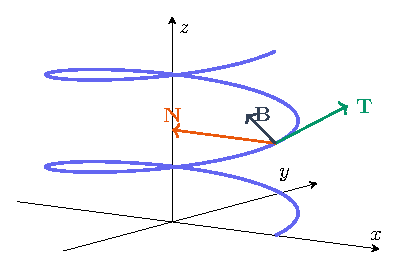
\includegraphics[width=.94\linewidth,height=65mm,keepaspectratio]{../assets/figures/helix.pdf}\par{\small\sffamily Uzay eğrisi üzerinde T teğet, N merkeze dönme yönü, B ise ikisine dik yönü gösterir.}\end{center}
\section{Eğrilik ve eğrilik yarıçapı}
Eğrilik, birim uzunluk başına teğet yönünün ne kadar değiştiğidir. Parametre daha hızlı ilerlediği için teğet daha hızlı değişebilir; bunu fiziksel hızdan ayırmak için \(d\mathbf T/dt\), \(ds/dt\) ile bölünür. Bir çemberde eğrilik yarıçapın tersidir.


{\small\[
\kappa=\left\|\frac{d\mathbf T}{ds}\right\|=\frac{\|\mathbf T\prime(t)\|}{\|\mathbf r\prime(t)\|}=\frac{\|\mathbf r\prime\times\mathbf r\prime\prime\|}{\|\mathbf r\prime\|^3},\qquad \rho=\frac1\kappa.
\]}
Düzlemde \(y=f(x)\) grafiği için \(\mathbf r(x)=(x,f(x),0)\) seçilirse \(\kappa=|f\prime\prime(x)|/[1+(f\prime(x))^2]^{3/2}\). Mutlak değer eğriliğin negatif olmamasını sağlar. Birim yay uzunluğuyla parametrelendirilmiş eğride \(\|d\mathbf r/ds\|=1\) ve \(\kappa=\|d^2\mathbf r/ds^2\|\).

\Needspace{10\baselineskip}\begin{tcolorbox}[title={Örnek 3.15 | Genel helisin eğriliği},colframe=accent]\(\mathbf r(t)=(a\cos t,a\sin t,bt)\), \(a>0\), için eğrilik nedir?
\par\vspace{1mm}{\scriptsize\sffamily Pekiştirme}\end{tcolorbox}
\begin{tcolorbox}[title={Adım adım çözüm},colback=green!3!white,colframe=green]\begin{enumerate}
\item \(\|\mathbf r\prime\|=\sqrt{a^2+b^2}\). \(\mathbf r\prime\times\mathbf r\prime\prime=(ab\sin t,-ab\cos t,a^2)\), normu \(a\sqrt{a^2+b^2}\).
\item \(\kappa=a/(a^2+b^2)\), \(\rho=(a^2+b^2)/a\). \(b=0\) olursa çember sonucu \(1/a\) elde edilir.
\end{enumerate}\end{tcolorbox}
Ek bilgi: eğrinin uzayda dönme düzleminin değişimini burulma ölçer. Yeterince türevlenebilir ve \(\mathbf r\prime\times\mathbf r\prime\prime\ne0\) iken \(\tau=[(\mathbf r\prime\times\mathbf r\prime\prime)\cdot\mathbf r\prime\prime\prime]/\|\mathbf r\prime\times\mathbf r\prime\prime\|^2\). Bu müfredatta temel hedef eğriliktir; burulma tamamlayıcıdır.

\section{Hız vektörü, sürat ve ivme}
Hız \(\mathbf v=\mathbf r\prime\) vektördür; sürat \(v=\|\mathbf v\|\) sayıdır. İvme \(\mathbf a=\mathbf v\prime\), hem süratin hem yönün değişmesini içerir. Sabit sürat sıfır ivme demek değildir: çembersel harekette yön değişir. \(\mathbf v\cdot\mathbf a=\tfrac12(v^2)\prime\) olduğundan hız ve ivmenin dikliği o anda süratin türevinin sıfır olmasıyla ilişkilidir.

\Needspace{10\baselineskip}\begin{tcolorbox}[title={Örnek 3.16 | Tahtadaki hareket örneği},colframe=accent]\(\mathbf r(t)=(5\cos t,5\sin t,6t^2)\). Hız, ivme ve bunların dik olduğu anı bulunuz.
\par\vspace{1mm}{\scriptsize\sffamily Ders fotoğrafından | \nolinkurl{IMG-20261015-WA0036.jpg}}\end{tcolorbox}
\begin{tcolorbox}[title={Adım adım çözüm},colback=green!3!white,colframe=green]\begin{enumerate}
\item \(\mathbf v=(-5\sin t,5\cos t,12t)\), \(\mathbf a=(-5\cos t,-5\sin t,12)\).
\item \(\mathbf v\cdot\mathbf a=25\sin t\cos t-25\sin t\cos t+144t=144t\). Yalnızca \(t=0\) anında diktirler.
\end{enumerate}\end{tcolorbox}
\Needspace{10\baselineskip}\begin{tcolorbox}[title={Örnek 3.17 | Üstel ve trigonometrik hareket},colframe=accent]\(\mathbf r(t)=(e^{-t},2\cos3t,2\sin3t)\). \(t=0\) anında hız, ivme büyüklükleri ve birim teğeti bulunuz.
\par\vspace{1mm}{\scriptsize\sffamily Ders fotoğrafından | \nolinkurl{IMG-20261015-WA0036.jpg}}\end{tcolorbox}
\begin{tcolorbox}[title={Adım adım çözüm},colback=green!3!white,colframe=green]\begin{enumerate}
\item \(\mathbf v=(-e^{-t},-6\sin3t,6\cos3t)\), \(\mathbf a=(e^{-t},-18\cos3t,-18\sin3t)\).
\item \(\mathbf v(0)=(-1,0,6)\), \(\|\mathbf v(0)\|=\sqrt{37}\); \(\mathbf a(0)=(1,-18,0)\), \(\|\mathbf a(0)\|=\sqrt{325}=5\sqrt{13}\).
\item \(\mathbf T(0)=(-1,0,6)/\sqrt{37}\). Vektörü büyüklüğüyle karıştırmamak için sonucun türünü kontrol et.
\end{enumerate}\end{tcolorbox}
\Needspace{14\baselineskip}\section{Fotoğraflardan ek eğri ve türev çözümleri}
\Needspace{10\baselineskip}\begin{tcolorbox}[title={Örnek 3.18 | Parametrik eğrinin türü},colframe=accent]\(\mathbf r(t)=(2+3t,4+5t,6+4t)\) eğrisinin türünü bulunuz.
\par\vspace{1mm}{\scriptsize\sffamily Ders fotoğrafından | \nolinkurl{IMG-20261009-WA0021.jpg}}\end{tcolorbox}
\begin{tcolorbox}[title={Adım adım çözüm},colback=green!3!white,colframe=green]\begin{enumerate}
\item \(\mathbf r(t)=(2,4,6)+t(3,5,4)\); sabit doğrultuda bir doğrudur.
\item Simetrik biçim \((x-2)/3=(y-4)/5=(z-6)/4\).
\end{enumerate}\end{tcolorbox}
\Needspace{10\baselineskip}\begin{tcolorbox}[title={Örnek 3.19 | Kapalı eğri ve uç teğetler},colframe=accent]\(\mathbf r(t)=(t^2-4,t^3-4t,0)\), \(-2\le t\le2\). Basit ve kapalı mıdır?
\par\vspace{1mm}{\scriptsize\sffamily Ders fotoğrafından | \nolinkurl{IMG-20261009-WA0025.jpg}}\end{tcolorbox}
\begin{tcolorbox}[title={Adım adım çözüm},colback=green!3!white,colframe=green]\begin{enumerate}
\item Her iki uç (0,0,0) olur. Farklı t ve s için eşit ilk koordinatlar s=-t gerektirir; ikinci koordinat eşitliği \(2t(t^2-4)=0\) verir.
\item Farklı parametrelerle tek tekrar uçlarda t=2 ve s=-2 dir; t=0 kendi kendine aynı parametredir. Dolayısıyla basit kapalı eğridir.
\item \(\mathbf r\prime=(-4,8,0)\) ve (4,8,0) uçlarda paralel değildir; kapama noktasında köşe vardır. Verilen parametrizasyon parçalı düzgün kapalı eğri olarak ele alınır.
\end{enumerate}\end{tcolorbox}
\Needspace{10\baselineskip}\begin{tcolorbox}[title={Örnek 3.20 | Türev ve ikinci türevin noktadaki değeri},colframe=accent]\(\mathbf r(t)=(1-\cos t,\sin t,t)\) için \(t=\pi/2\) anındaki ilk iki türevi bulunuz.
\par\vspace{1mm}{\scriptsize\sffamily Ders fotoğrafından | \nolinkurl{IMG-20261009-WA0024.jpg}}\end{tcolorbox}
\begin{tcolorbox}[title={Adım adım çözüm},colback=green!3!white,colframe=green]\begin{enumerate}
\item \(\mathbf r\prime=(\sin t,\cos t,1)\), \(\mathbf r\prime\prime=(\cos t,-\sin t,0)\).
\item Noktadaki değerler (1,0,1) ve (0,-1,0). Teğet noktası \((1,1,\pi/2)\), teğet doğrusu bu noktadan (1,0,1) yönünde geçer.
\end{enumerate}\end{tcolorbox}
\Needspace{10\baselineskip}\begin{tcolorbox}[title={Örnek 3.21 | Vektörel çarpımın türevini iki yoldan almak},colframe=accent]\(\mathbf U=(t,-t,t^2/2)\), \(\mathbf V=(t^4/4,t^3/3,t^2/2)\). Çarpımın türevini bulunuz.
\par\vspace{1mm}{\scriptsize\sffamily Ders fotoğrafından | \nolinkurl{IMG-20261009-WA0024.jpg}}\end{tcolorbox}
\begin{tcolorbox}[title={Adım adım çözüm},colback=green!3!white,colframe=green]\begin{enumerate}
\item Önce çarpım: \(\mathbf U\times\mathbf V=(-t^3/2-t^5/6,t^6/8-t^3/2,t^4/3+t^5/4)\).
\item Türev \((-3t^2/2-5t^4/6,3t^5/4-3t^2/2,4t^3/3+5t^4/4)\).
\item Alternatif \(\mathbf U\prime\times\mathbf V+\mathbf U\times\mathbf V\prime\) aynı sonucu verir. Orta bileşenin t altıncı kuvvetinin türevi \(6t^5/8=3t^5/4\); defterdeki bu satır sadeleştirilerek kontrol edildi.
\end{enumerate}\end{tcolorbox}
\Needspace{10\baselineskip}\begin{tcolorbox}[title={Örnek 3.22 | Sabit normun türevi},colframe=accent]\(\mathbf r(t)=(a\cos t,a\sin t,0)\), a>0, için hızın konuma dik olduğunu kanıtlayınız.
\par\vspace{1mm}{\scriptsize\sffamily Ders fotoğrafından | \nolinkurl{IMG-20261015-WA0036.jpg}}\end{tcolorbox}
\begin{tcolorbox}[title={Adım adım çözüm},colback=green!3!white,colframe=green]\begin{enumerate}
\item \(\mathbf r\prime=(-a\sin t,a\cos t,0)\); konumla çarpım \(-a^2\sin t\cos t+a^2\sin t\cos t=0\).
\item Genel gerekçe: \(\mathbf r\cdot\mathbf r=a^2\) sabit olduğundan türevi \(2\mathbf r\cdot\mathbf r\prime=0\).
\end{enumerate}\end{tcolorbox}
\section{İvmenin teğetsel ve normal bileşenleri}
\(\mathbf v=v\mathbf T\) ifadesinin türevi alınırsa ivmenin bir kısmı sürati, diğer kısmı yönü değiştirir. Normal bileşen, eğriliğin ve süratin karesinin çarpımıdır. Teğetsel katsayı negatif olabilir; normal katsayı negatif değildir.


{\small\[
\mathbf a=\frac{dv}{dt}\mathbf T+\kappa v^2\mathbf N,\qquad a_T=\frac{\mathbf v\cdot\mathbf a}{\|\mathbf v\|},\qquad a_N=\frac{\|\mathbf v\times\mathbf a\|}{\|\mathbf v\|}.
\]}
\Needspace{10\baselineskip}\begin{tcolorbox}[title={Örnek 3.23 | Dairesel harekette ivme},colframe=accent]\(\mathbf r(t)=(a\cos\omega t,a\sin\omega t,0)\), \(a>0,\omega\ne0\) için \(a_T,a_N\) nedir?
\par\vspace{1mm}{\scriptsize\sffamily Pekiştirme}\end{tcolorbox}
\begin{tcolorbox}[title={Adım adım çözüm},colback=green!3!white,colframe=green]\begin{enumerate}
\item Sürat \(a|\omega|\) sabit olduğundan \(a_T=0\). Eğrilik \(1/a\).
\item \(a_N=(1/a)(a^2\omega^2)=a\omega^2\). İvme tamamen içeriye yönelir; sürat sabit olmasına rağmen sıfır değildir.
\end{enumerate}\end{tcolorbox}
\begin{enumerate}
\item Önce türevlerle hız ve ivmeyi bul; sonra norm al.
\item Frenet çatısı istenirse her vektörün birim ve diğerlerine dik olduğunu kontrol et.
\item Yay uzunluğunda integralin içine norm, eğrilikte normun küpünü yaz.
\item Normal ve binormal için sıfır eğrilik olasılığını kontrol et.
\end{enumerate}

\clearpage
\section*{Kaynaklar ve kapsam}
\addcontentsline{toc}{section}{Kaynaklar ve kapsam}
Bu metin 156 ders/defter fotoğrafı ve altı başlıklı müfredata göre özgün olarak yazıldı. Fotoğraflar dersin sıra ve örneklerini belirler. Ek sorular pekiştirme olarak etiketlidir; çıkmış sınav sorusu iddiası yoktur. Soluk semboller tahminle aktarılmadı. Gradyan ve yönlü türev, müfredat gereği tamamlanan anlatımdır. Fotoğraf bazında inceleme dizini web sitesinde ve analysis/FOTOGRAF\_INCELEMESI.md dosyasında bulunur.
\textbf{Birincil ders malzemesi}. Kullanıcının sağladığı 156 JPG ders/defter fotoğrafı ve mufredat.png. Dosya tarihleri ders tarihi olarak varsayılmadı. Konu-fotoğraf eşleştirmesi fotoğraf dizinindedir.\par
\textbf{Erwin Kreyszig · Advanced Engineering Mathematics}. Dersin belirtilen kitabı. Wiley 10. baskı bölüm diziniyle vektör diferansiyel hesabı başlığı eşleştirildi; tam kitap dosyası sağlanmadı. Kitaptan birebir metin veya soru aktarımı yapılmadı.
{\footnotesize\url{https://bcs.wiley.com/he-bcs/Books?action=contents&bcsId=6140&itemId=0470458364}}\par
\textbf{KOCW · Kreyszig temelli Bölüm 9 ders notları}. Sungkyunkwan / Kim Munhyeon, vektörler ve vektör fonksiyonları. Açık üniversite notu kavram ve formül kontrolünde kullanıldı. Buradaki Türkçe açıklamalar ve çözümler özgün olarak yazıldı.
{\footnotesize\url{https://contents.kocw.net/KOCW/document/2015/sungkyunkwan/kimmunhyeon3/8.pdf}}\par
\textbf{Zill ve Wright · Calculus / Matematik}. Kullanıcının verdiği bibliyografya: İ. N. Cangül çevirisi, Nobel, 2013. Tam metne erişilmedi; baskıya özgü sayfa ve soru numarası atfedilmedi.\par
\textbf{Mustafa Balcı · Genel Matematik II}. Kullanıcının verdiği bibliyografya: Sürat, 2013. Tam metin sağlanmadı; bu kitaptan doğrulanmış alıntı veya sayfa atfı yapılmadı.\par
\textbf{MIT OCW · 18.02 ders notları}. Denis Auroux, 2007. Ders düzeni ve kavram denetimi için açık ders dizini. Müfredat dışındaki çok katlı integraller ve integral teoremleri bu çalışmaya eklenmedi.
{\footnotesize\url{https://ocw.mit.edu/courses/18-02-multivariable-calculus-fall-2007/pages/lecture-notes/}}\par
\textbf{MIT · Teğet düzlem ve gradyan}. Gradyanın teğet düzlem ve yönlü türevle ilişkisi için açık teknik kontrol kaynağı. Konuya eklenen örnekler özgün pekiştirme sorularıdır.
{\footnotesize\url{https://www.ocw.mit.edu/ans7870/18/18.013a/textbook/HTML/chapter06/section05.html}}\par
\end{document}
